% !TEX root = ../Seminararbeit-Data_Mining_Frameworks.tex
%


% =============================================================================
%
% Datensatz und Beispiel-Modell
%
% =============================================================================
\chapter{Datensatz und Beispiel-Modell}
\label{sec:example}

\section{Datensatz}
\label{sec:example:data}

\begin{figure}[htb]
	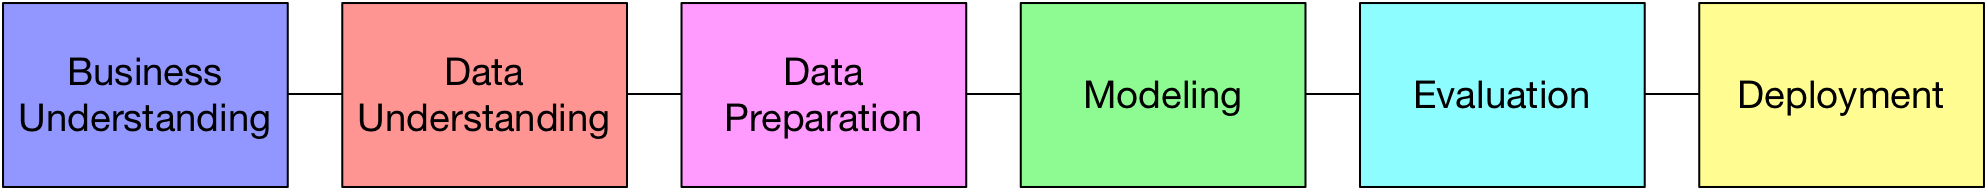
\includegraphics[width=\textwidth]{gfx/crisplinear.png}
	\caption{Der CRISP-DM Prozess als Kette der einzelnen Schritte}
	\label{fig:example:data:crisp}
\end{figure}

Für die Umsetzung des Beispiels wurde der Eingangs bereits beschriebene CRISP-DM
Data Mining Prozess verwendet. Die Daten wurden gemäß den 6 Schritten „Business
Understanding“, „Data Understanding“, „Data Preparation“, „Modeling“,
„Evaluation“ und „Deployment“ verarbeitet.

\subsection{Business Understanding}
\label{sec:example:data:bu}

Als Datengrundlage für das Beispiel dienen die Daten der
Veranstaltungsevaluationen der Vergangenen Semester, durchgeführt von der
Fachschaft Mathematik, Physik und Informatik der Universität Bayreuth. Mithilfe
der vorliegenden Datengrundlage sollen nun folgende Fragen beantwortet werden:

\begin{itemize}
  \item „Warum beschweren sich einige Studenten, während andere die Veranstaltung
  super finden? Bzw. welche Ursachen gibt es für eine Beschwerde?“
  \item „Wie sind die Prognosen für die bevorstehenden Evaluationen?“
\end{itemize}

\subsection{Data Understanding}
\label{sec:example:data:du}

Im nächsten Schritt ist es wichtig herauszufinden, wie die Daten erhoben wurden.
Im Beispiel der Veranstaltungsevaluationen ist dies durch austeilen eines
Fragebogens erfolgt.

\begin{figure}[htb]
	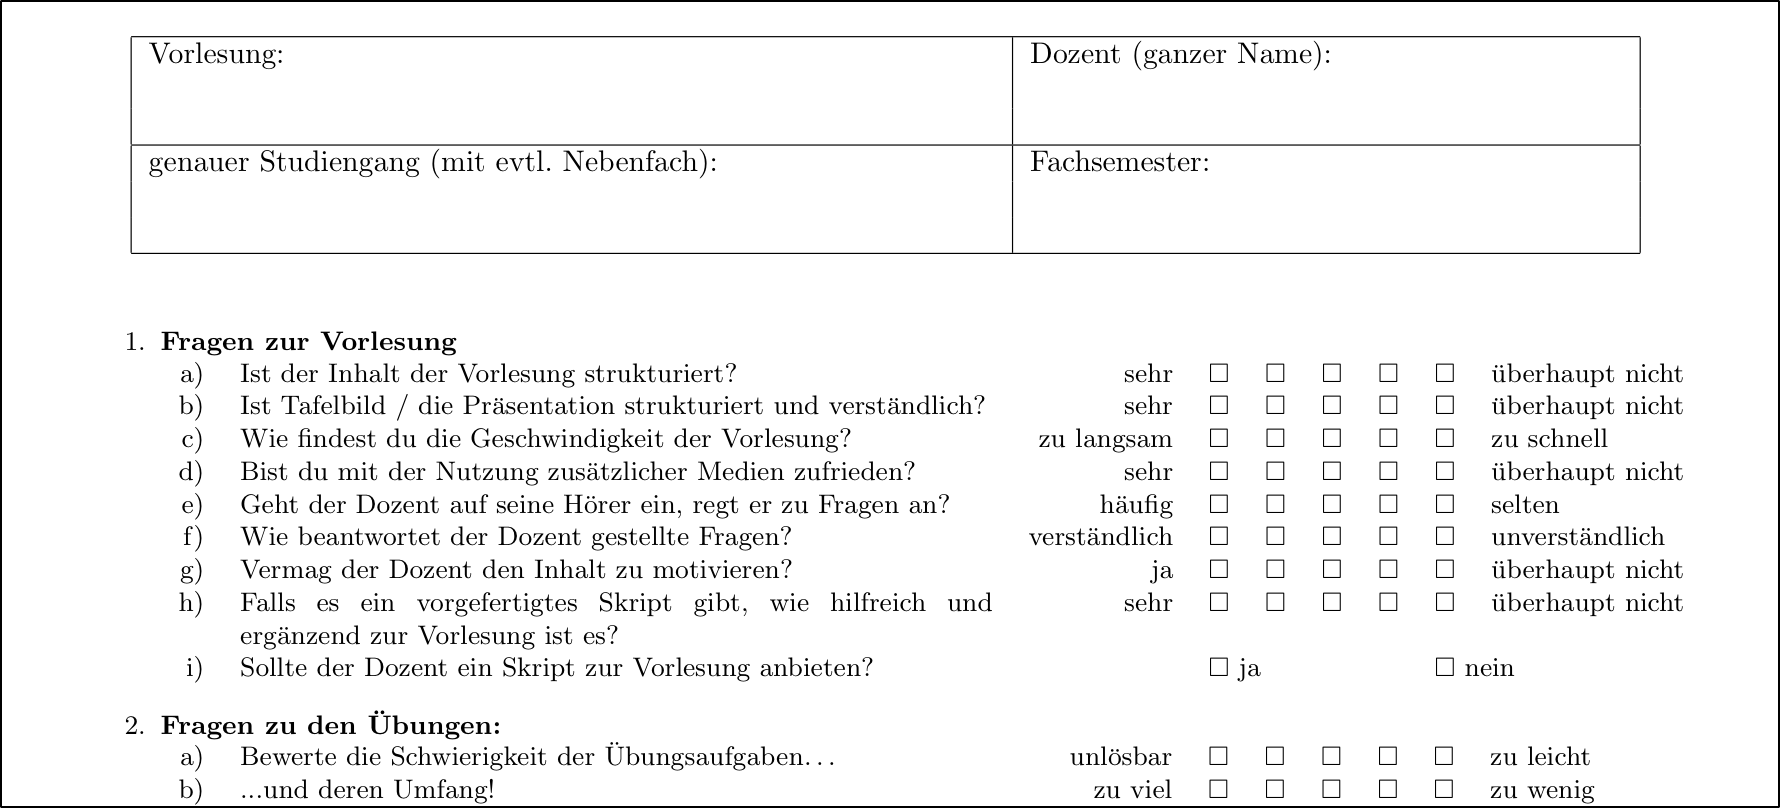
\includegraphics[width=\textwidth]{gfx/questionnaire.png}
	\caption{Fragebogen, zur Erhebung der Evaluationsdaten}
	\label{fig:example:data:du:qu}
\end{figure}

Anhand des Fragebogens erkennt man, dass die Antwortmöglichkeiten in Form von
anzukreuzenden Kästchen gegeben waren. Jedes Kreuz repräsentiert dabei einen
Wert im Bereich von 0 bis max. 4. \\
Außerdem muss festgestellt werden, wie die Daten in der Datenbank abgelegt
werden. Hierfür kann man bspw. ein ER-Diagramm erzeugen oder sich eine Vorschau
der Daten in Form einer Tabelle generieren lassen.

\begin{figure}[htb]
  \center
	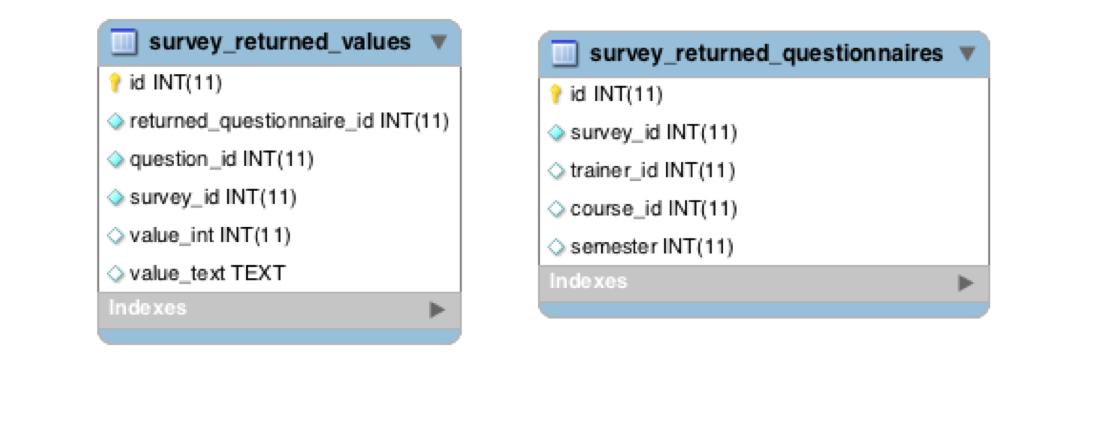
\includegraphics[width=0.7\textwidth]{gfx/db1.png}
  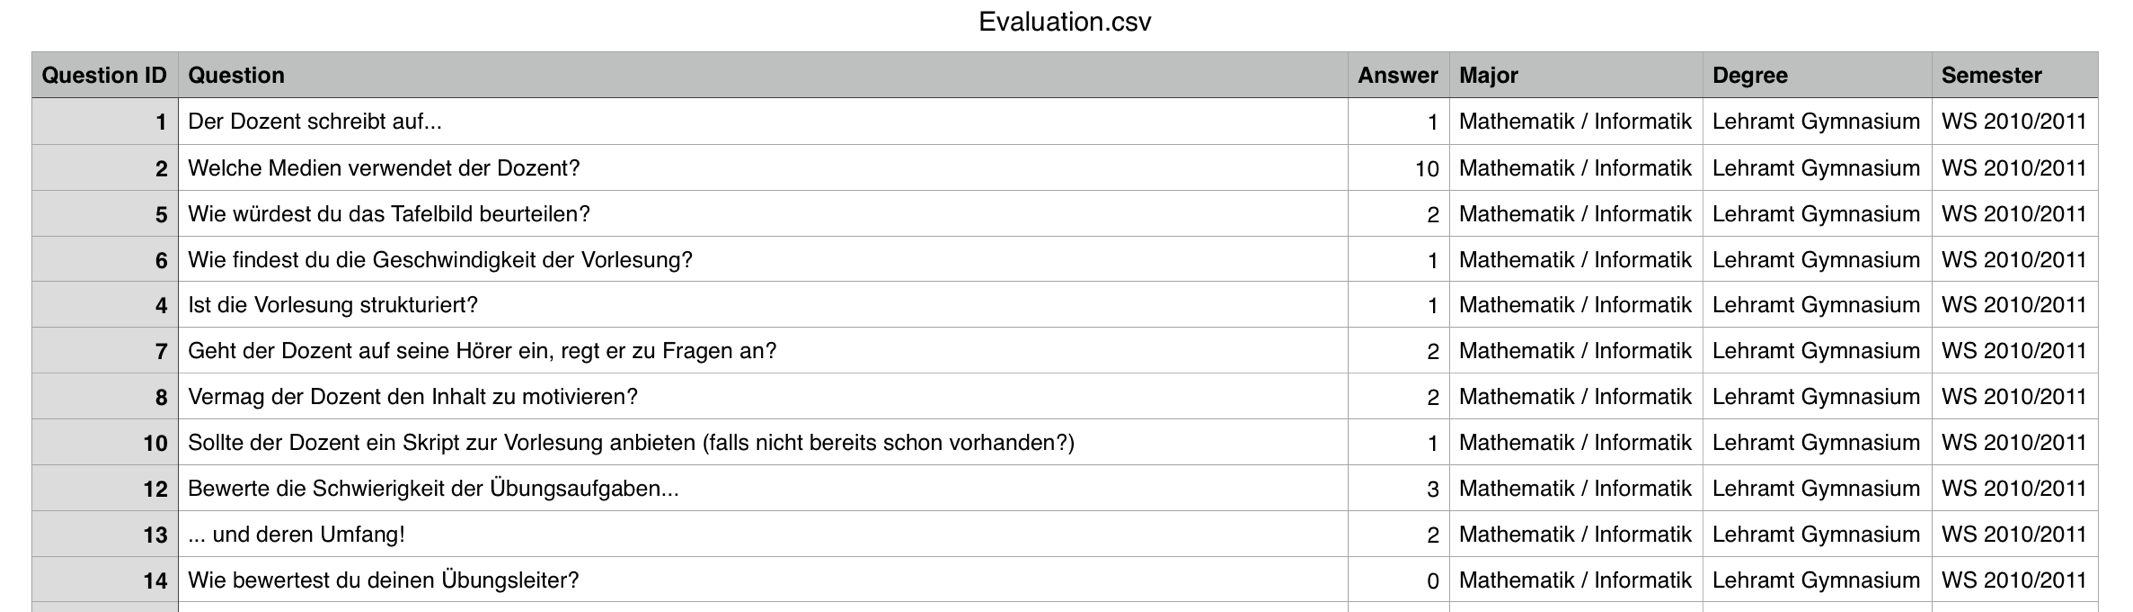
\includegraphics[width=\textwidth]{gfx/db2.png}
	\caption{Repräsentation der Daten in der Datenbank}
	\label{fig:example:data:du:db}
\end{figure}

Mithilfe dieser Informationen erkennt man, dass sich die gesuchten Daten in den
beiden Tabellen „survey\_returned\_values“ und „survey\_returned\_questionnaires“
befinden und wie diese strukturiert sind.

\subsection{Data Preparation}
\label{sec:example:data:dp}

Wurden nun die entsprechenden Tabellen bzw. deren Attribute festgelegt müssen
diese nun im nächsten Schritt aus der Datenbank extrahiert werden um separat
Analysiert werden zu können. Dies geschieht mit der folgenden SQL-Abfrage.

\begin{figure}[htb]
	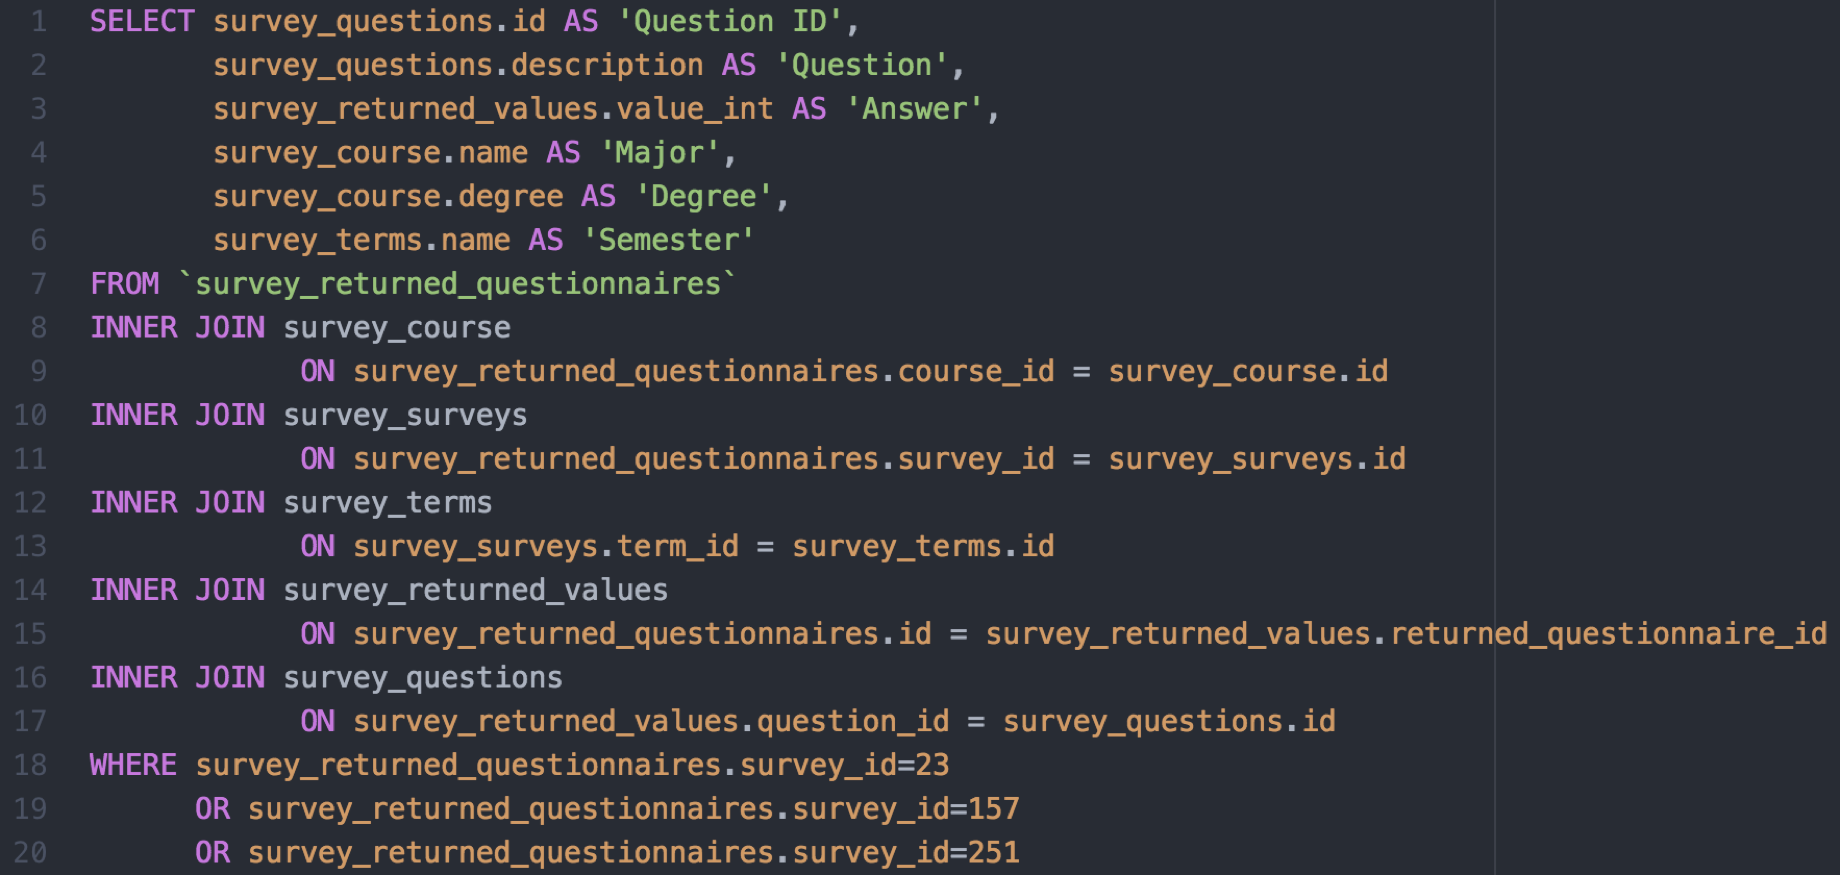
\includegraphics[width=\textwidth]{gfx/sql.png}
	\caption{SQL Anfrage für den Export der Daten}
	\label{fig:example:data:dp:sql}
\end{figure}

Die Ergebnisdatensätze der SQL-Abfrage können nun als .csv Datei exportiert
werden um danach in der jeweiligen Data Mining Software verarbeitet werden zu
können.

\subsection{Modeling}
\label{sec:example:data:mod}

In der Modellierungsphase muss nun ein Algorithmus gewählt werden, welcher die
vorbereiteten Daten so verarbeiten kann, dass die Anfangs definierten
Fragestellungen beantwortet werden können. In unserem Beispiel eignet sich die
Frage nach der Gesamtnote, da dieses Attribut eine gute Repräsentation der
Gesamtbewertung für eine Veranstaltung darstellt. \\
Es muss also ein Algorithmus gewählt werden, welcher nach einem einzelnen
Attribut, dem sog. Label, Daten Mined. Ein einfach auszuwertender Algorithmus,
der genau diese Voraussetzungen erfüllt ist der sog. „Entscheidungsbaum“
(engl.: „Decision Tree“).

\begin{figure}[htb]
  \center
	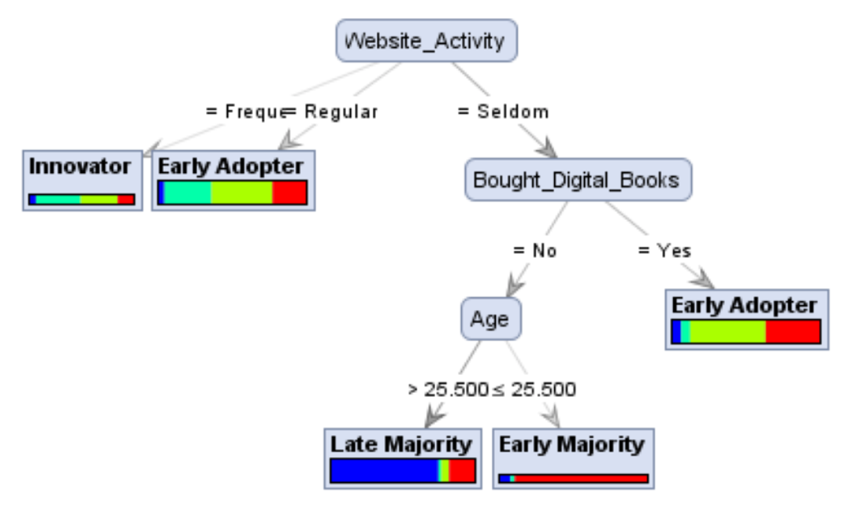
\includegraphics[width=0.5\textwidth]{gfx/dt.png}
	\caption{Beispiel für einen Entscheidungsbaum \cite{North:2012}}
	\label{fig:example:data:mod:dt}
\end{figure}

Die Knoten des Baumes stellen klassifizierende Attribute des Ausgangs-Datensatzes
dar, während die Blätter die möglichen Werte des Labels anzeigen. Außerdem
zeigen die Blätter noch an, auf wieviel Datensätzen die jeweilige Klasse beruht.

\subsection{Evaluation + Deployment}
\label{sec:example:data:eval}

Schließlich kann mithilfe des „Decision Trees“ ermittelt werden, dass
beispielsweise das Studienfach oder ein bestimmtes Semester die Ursache für
vermehrte Beschwerden (respektive mehrere schlechte Bewertungen) waren.
Gleichzeitig kann man mit den entsprechenden Informationen über Studienfach,
Abschluss etc. der aktuellen Kursteilnehmer eine Prognose für die bevorstehende
Lehrveranstaltungsevaluation abgeben.

\section{Umsetzung}
\label{sec:example:impl}

\subsection{Rapidminer Studio}
\label{sec:example:impl:rm}

\subsection{Microsoft Azure Machine Learning Studio}
\label{sec:example:impl:msa}
